%%% The main file. It contains definitions of basic parameters and includes all other parts.


%% Settings for two-sided (duplex) printing
\documentclass[12pt,a4paper,twoside,openright]{report}
\let\openright=\cleardoublepage

%% Character encoding: usually latin2, cp1250 or utf8:
\usepackage[utf8]{inputenc}


%% Further useful packages (included in most LaTeX distributions)
\usepackage{amsmath}        % extensions for typesetting of math
\usepackage{amsfonts}       % math fonts
\usepackage{amsthm}         % theorems, definitions, etc.
%\usepackage{bbding}         % various symbols (squares, asterisks, scissors, ...)
%\usepackage{bm}             % boldface symbols (\bm)
\usepackage{graphicx}       % embedding of pictures
\usepackage{caption}       % embedding of pictures
\usepackage{subcaption}       % embedding of pictures
%\usepackage{fancyvrb}       % improved verbatim environment
%\usepackage[square]{natbib}         % citation style AUTHOR (YEAR), or AUTHOR [NUMBER]
%\usepackage[nottoc]{tocbibind} % makes sure that bibliography and the lists
			    % of figures/tables are included in the table
			    % of contents
%\usepackage{dcolumn}        % improved alignment of table columns
\usepackage{tikz}
%\usetikzlibrary{shapes,fit,positioning,snakes,mindmap,trees,decorations.text,arrows.meta}
\usepackage{nomencl}
\usepackage{epigraph}
\makenomenclature
\usepackage{algorithm,algpseudocode}
\usepackage{enumitem}
\usepackage{booktabs}
\usepackage{mwe}

\usepackage{listings}
\lstset{basicstyle=\ttfamily,
	showstringspaces=false,
	commentstyle=\color{red},
	keywordstyle=\color{blue}
}

\usepackage{pdfpages}

\usepackage[textsize=tiny]{todonotes}
\usepackage[a-2u]{pdfx}
\setitemize{itemsep=0pt}
%\usepackage[usenames]{xcolor}  % typesetting in color
\usepackage[textsize=tiny]{todonotes}
\newcommand{\XX}[1]{\textcolor{red}{#1}}
\newcommand{\X}[1]{\textsc{#1}}
%%% Basic information on the thesis

% Thesis title in English (exactly as in the formal assignment)
\def\ThesisTitle{Traffic scheduler \\ \vspace{5mm} for Differentiated Services}

% Author of the thesis
\def\ThesisAuthor{Michal Bali}

% Year when the thesis is submitted
\def\YearSubmitted{2018}

% Name of the department or institute, where the work was officially assigned
% (according to the Organizational Structure of MFF UK in English,
% or a full name of a department outside MFF)
\def\Department{Department of Software Engineering}

% Is it a department (katedra), or an institute (ústav)?
\def\DeptType{Department}

% Thesis supervisor: name, surname and titles
\def\Supervisor{Miroslav Kratochvíl, M.Sc.}

% Supervisor's department (again according to Organizational structure of MFF)
\def\SupervisorsDepartment{Department of Software Engineering}

% Study programme and specialization
\def\StudyProgramme{Computer Science}
\def\StudyBranch{General Computer Science}

\setlength\epigraphwidth{9cm}
\setlength\epigraphrule{0pt}

% An optional dedication: you can thank whomever you wish (your supervisor,
% consultant, a person who lent the software, etc.)
\def\Dedication{%

%\epigraph{}

%\noindent

%\emph{}.

%\vspace{3 ex}
%\noindent
I would also like to thank my supervisor Mirek Kratochvíl.
}

% Abstract (recommended length around 80-200 words; this is not a copy of your thesis assignment!)
\def\Abstract{%
Lorem ipsum
}

% 3 to 5 keywords (recommended), each enclosed in curly braces
\def\Keywords{%
{computer networks,} {internet,} {network traffic scheduling,} {active queue management}
}



%% The hyperref package for clickable links in PDF and also for storing
%% metadata to PDF (including the table of contents).
%\usepackage[pdftex,unicode]{hyperref}   % Must follow all other packages
%\hypersetup{breaklinks=true}
%\hypersetup{pdftitle={\ThesisTitle}}
%\hypersetup{pdfauthor={\ThesisAuthor}}
%\hypersetup{pdfkeywords=\Keywords}
%\hypersetup{urlcolor=blue}

% Definitions of macros (see description inside)
\include{macros}

% Title page and various mandatory informational pages
\begin{document}
\include{title}

%%% A page with automatically generated table of contents of the bachelor thesis

\tableofcontents

%%% Each chapter is kept in a separate file
\chapter*{Introduction}
\addcontentsline{toc}{chapter}{Introduction}

Lorem

\section*{Motivation}
\addcontentsline{toc}{section}{Motivation}


\section*{Goals}
\addcontentsline{toc}{section}{Goals}


\section*{Related Work}
\addcontentsline{toc}{section}{Related Work}

\subsection*{Related Research}
\addcontentsline{toc}{subsection}{Related Research}


\subsection*{Similar Software}
\addcontentsline{toc}{subsection}{Similar Software}


\section*{Layout of this Thesis}
\addcontentsline{toc}{section}{Layout of this Thesis}


\chapter{Traffic scheduling}
\label{chap:gf}

Internet is growing -> people depend more and more on it - its harder to maintain QoS.

 QoS - that is bandwidth allocation (fairness for all, because clients share some limits), acceptable delay(jitter)
 
ISP - klienti si platia za nejaku kvalitu

co je to traffic scheduling - stoji medzi 2-3 layer OSI, mby trosku HW popisat? netdevice queue vs queing discipline 

\section{Bufferbloat}


In gateways of packet-switched networks, short-term differences between arrival and departure rate naturally happen. To balance these bursts, buffers are used - packets are waiting in queues until they can be sent towards their destination. This helps avoiding outgoing link starvation and increases throughput. Without buffers, the gateway has no place to store incoming packets and they get dropped, which decrease throughput.


However, the more packets are in a queue, the longer packets stay in it and the longer it takes to be delivered. Unfortunately, queues in modern networks tend to fill up and stay 'bloated' \cite{Gettys:2012:BDB:2063176.2063196}. That means some amount of packets always stay in the queue (it never becomes empty), even if there are no incoming bursts to balance.

\begin{figure}
	\centering

\includegraphics[width=137mm]{drawings/tcp_no_bottleneck}
\caption{TCP without bottleneck. The grey rectangles are packets. Horizontal dimension is time, vertical is bandwidth. That means the area of rectangle is size of packet.}

\label{fig01:no_bottle}
\end{figure}

To understand why queues become bloated, let's take a look at Transport Control Protocol (TCP), which is the most widely used layer 4 protocol. It achieves its reliability with following policy: After packet is transmitted, receiver sends an ACK packet back to sender to let him know which packets have been successfully received and which must be resent. But waiting on ACK after each packet would provide miserable throughput and most of the time both sides would wait on single packet. The sender goes ahead and transmit packets without getting ACKs on previous ones. This fills the whole route, so at all times one packet is being sent, one packet is being received. The ACKs that are coming back retain the same spacing. The situation is displayed on Figure \ref{fig01:no_bottle}.

Figure \ref{fig01:no_bottle} shows connection with constant bandwidth along whole path, which is rarely the case in today's Internet. Typical path consists of many hops with links of different bandwidth. That means somewhere must be a bottleneck - link with lowest bandwidth. If the sender transmitted at the rate of adjacent link, the network would become congested. Bottleneck link would not be able to forward all incoming traffic, its buffer would fill, and the rest of arriving packets would be dropped. That actually induces even more traffic, because sender would try to resend dropped packets.


%tcp by potrebovalo vediet aky badwidth ma bottleneck
TCP must limit upstream rate. In ideal case, it would work at the rate of slowest link. However, the sender does not have any information about bottleneck whatsoever. TCP uses congestion window: it is amount of bytes TCP can send without receiving an ACK. When an ACK is received, it frees space in congestion window, and next packet can be sent, filling the window again. The first ACK is received after round trip time (RTT) - the time it takes to transmit packet on path sender-receiver-sender.

To maximize throughput, size of congestion window should be at least the (bottleneck) bandwidth-delay product (product of bandwidth and RTT) bytes. In this case, the sender fills the pipe with packets just before it receives first ACK and is allowed to send following packets. On the other hand, if congestion window exceeds the bandwidth-delay product, the excessive packets stay in queues along the path and cause delay. 

%TCP uses slow start algorithm to find ideal congestion window at start, and then congestion control algorithm takes over to maintain it near the inflection point of maximized throughput and minimizing delay. This if solution to avoiding congestion collapse, but the Internet encounters problem of persistently full buffers - bufferbloat.



Bufferbloat is caused by mismatch between congestion window and actual RTT \cite{CoDel}. In reality, estimating the window size is difficult. Always-changing network load affect both RTT and bandwidth, paths change thanks to rerouteing. Buffers can really only be measured at the bottleneck and even there it is hard to differentiate between useful and useless buffers that only cause delay.

\begin{figure}
	\centering
	\includegraphics[width=137mm]{drawings/tcp_bottleneck_1}
	\caption{Start of TCP communication.}
	
	\label{fig02:bottle_1}
\end{figure}


Figure \ref{fig02:bottle_1} shows a starting TCP communication. Illustrated network consists of 3 subnetworks. The left and right have bandwidth 30 Mb/s, the middle one has 10 Mb/s. One packet has 30kb. TCP Congestion window is 20 packets. The sender starts by transmitting whole window of packets back to back. They arrive at edge of bottleneck network and get enqueued there, because of bandwidth difference. A packet arrives from left network every 1 ms, but only every 3 ms is one dequeued. On the right side, they retain spacing given by bottleneck as shown in Figure \ref{fig03:bottle_2}. The receiver turns incoming packets into ACKs with the same spacing. The sender then sends one packet of data for each ACK it gets.

This way, after one RTT, whole connection has gotten into state of equilibrium. The bottleneck is fully utilized, so the throughput is as high as possible. However, a queue at the middle network will never be empty. At first, it had to hold the burst of whole congestion window. Once all 20 packets were sent, 14 of them were waiting in the queue, 6 had already been forwarded to middle network. Then, no packets were enqueued and every 3 ms one was dequeued. Until one RTT passed, first ACK was delivered and next packet sent into left network. After that, every 3 ms one packet arrives and one leaves. 5 packets stay there and every one of them waits long 15 milliseconds. Also, they block buffer space other connections could use. 

\begin{figure}
	\centering
	\includegraphics[width=137mm]{drawings/tcp_bottleneck_2}
	\caption{TCP after one RTT}
	
	\label{fig03:bottle_2}
\end{figure}

The queue stayed in the buffer in figure  \ref{fig03:bottle_2} because congestion window was set to 5 more packets than the bandwidth-delay product. Determining the size is not an easy task. At start of TCP, slow start algorithm \cite{Jacobson:1988:CAC:52324.52356} is used to determine size of congestion window. It grows exponentially, increasing size of window with each ACK received, until a threshold is reached or packet is dropped.  After that, congestion avoidance takes over to maintain it. Over the years of TCP in service, many variants were introduced. Currently CUBIC [ref] is used widely. 

%emhasize that it is a way to communicate
Congestion windows are managed by TCP endpoints, while congestion and bufferbloat takes place in gateways along the path. There is no direct communication channel between them. When the buffer becomes full, the next packets must be dropped simply because there is no room for them. When TCP does not receive an ACK, it the congestion avoidance algorithm reduces the window and slows down.

Relatively new is Explicit Congesion Notification (ECN) \cite{rfc3168:ECN}. There are 2 bits reserved for ECN in IP header, so packets may be marked, that there is ongoing congestion. Both sides have to support ECN  - the receiver has to read the 2 bits and send ACK with the same bits back. The sender then may react like ACK didn't arrive at all. In May 2017, passive support for ECN was available on 70 \% of popular websites \cite{ECN:proceedings}.

This all indicated, that simple tail drop queues, which drop packets only when they are full may be superseded by more sophisticated queues right in the gateways. It involves the counter-intuitive idea of dropping perfectly good packets even if buffer is not full yet. But it indicates a problem, while still having room for balancing bursts. This approach is called Active Queue Management (AQM), and is recommended to use throughout the Internet.


\subsection{RED}

%kde sa nachadza queue management?

\begin{figure}
	\centering
	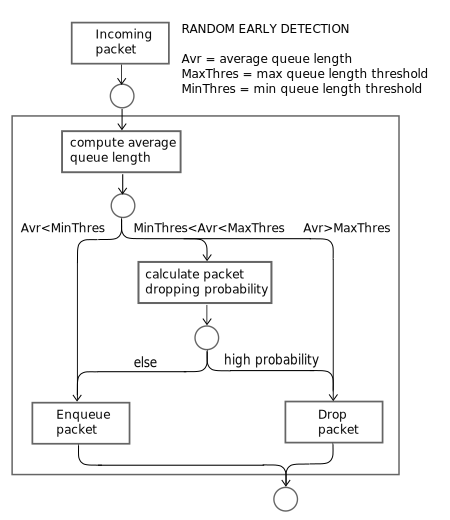
\includegraphics[width=137mm]{drawings/RED}
	\caption{The Random Early Drop algorithm \cite{RED:picture} }
	
	\label{fig04:RED}
\end{figure}

In 1993, Sally Floyd and Van Jacobson introduced Random Early Drop (RED) \cite{Floyd:1993:RED:169931.169935}. It monitored average length of queue. According to it, it may drop (mark) incoming packet with certain (possibly 100 \%) probability, which is function of average. It addressed congestion avoidance problem as well as TCP synchronization problem, that were encountered using tail drop. However, it had quite a few parameters, which have to be set differently in various networks. Without this tuning, it functioned poorly which led to general reluctance of deployment, although it was recommended by Internet Engineering Task Force \cite{rfc2309} in 1998.

To determine the average, RED uses exponential weighted moving average:
\[
avg := (1 - w_q)avg+w_qq.
\]
$q$ is number of packets in queue and $w_q$ is parameter of RED that represents degree of weighting decrease, or how much the average responds to new packets and how much weight have the past states. Too high $w_q$ would mean bias against short bursts. With lower $w_q$, average is more fluid and queue responds to congestion slower.

At each enqueue, the $avg$ is compared to two parameters $min_{th}$ and $max_{th}$, as showed on Figure \ref{fig04:RED}. If it lower than $min_{th}$, packet is just enqueued as is. If $avg$ is higher than $max_{th}$, the packet is marked (dropped). This ensures, that if endpoints respond to marking properly, or packets are actually dropped, number of packets in queue will not exceed maximum for long.

If $avg$ is between the thresholds $min_{th}$ and $max_{th}$, packet is marked (dropped) with probability $p_a$, that is function of the average and . Let $p_b$ be linear function of $avg$ that varies from 0 to $max_p$ ($max_p$ is parameter of RED):
\[
  p_b = max_p \frac{(avg - min_{th})}{max_{th} - min_{th}}.
\]
Further, the final marking probability $p_a$ depends on when was the last packet marked (dropped):
\[
p_a = \frac{p_b}{1-count \cdot p_b},
\]
where $count$ is number of packets that were enqueued since the last mark (drop). This ensures, that dropped packets will never be too far, nor too close \cite[Section 7]{Floyd:1993:RED:169931.169935}.

RED also has option to work based on number of bytes in buffer instead number of packets. In this case:
\[
  p_b = max_p \frac{(avg - min_{th})}{max_{th} - min_{th}}
\]\[
  p_b = p_b \frac{size_{packet}}{size_{max}}
\]\[
  p_a = \frac{p_b}{1-count \cdot p_b},
\]
where $size_{packet}$ is size of packet being enqueued and $size_{max}$ is maximum size of packet. This way, large packets are more likely to get marked, and probability corresponds more precisely to actual time that packet spend in queue.

%!!!!!!!!!!!!!!!!!!je v pohode tam dat takyto odstavec o ktorom neviem vela??
Over the years, several variants of RED have been introduced. With Weighted RED different packets have different probability functions for different classes of traffic (classified for example by DSCP). Adaptive RED \cite{Floyd01adaptivered:} tunes the RED algorithm to remove sensitivity to some of the parameters. Robust RED \cite{RRED} was proposed to counter low-rate Denial-of-Service attacks.

\subsection{CoDel}

In 2012, Jacobson and Nichols introduced Controlled Delay - CoDel \cite{CoDel}. Their AQM uses local minimum length of queue as indication of bufferbloat. Additionally, it works only with sojourn time - the time packet spends in queue. That means it is independent of bandwidths of adjacent links, because it only works with time - if it is deployed in a backbone, with 10 Gb/s bandwidth, acceptable queue will be 50 Mb big. On the other hand on slow links, say 10 Mb/s, corresponding acceptable buffer is only 50 kb. CoDel measures time packets spend in queue and if it exceeds a threshold for a longer time, it starts to drop packets.

It has 2 parameters:
\begin{itemize}
	\item $Target$ is the target delay CoDel tries to keep. Defaults at 5 ms.
	\item $Interval$ sets period of time for which it is OK exceed $Target$. Defaults at 100 ms.
\end{itemize}
So CoDel drops packets, if packets spend more than $Target$ time in queue for more than $Interval$ time. Also, CoDel does not drop packets, if fewer that MTU (Maximum Transmission Unit) worth of bytes is in queue.

Every time a packet arrives, a time stamp is tagged to it. At dequeue, CoDel looks how long was the dequeued packet in queue. If packets have exceeded the $Target$ time for at least $Interval$, CoDel enters dropping state. In this state, packets are dropped at an increasing rate until the sojourn time of packets at front is lower than $Target$. The next drop time is calculated as follows:
\[
  DropInterval = \frac{Interval}{\sqrt{count}},
\]
where count is number of packets dropped since dropping state entry and DropInterval is time after next packet will be dropped.







\section{fairness -> SFQ}x
-vyhody pristupu jeden flow - jeden queue

- SFQ - hashovanie


\subsection{DRR}
-DRR je fair

-fq\_codel = CoDel + SFQ + DRR

\section{Bandwidth allocation}

-TBF - HFSC

\section{Differentiated services}
-classes of traffic
?


\chapter{Our traffic scheduler}
\label{chap02}
%motivation: little config (knobless), fast O(1), QoS aware, scheduler in presence of differentiated services. Would run at simple devices

\begin{figure}
	\centering
	\includegraphics[width=137mm]{drawings/msfc}
	\caption{The MSFC layout}
	\label{fig10:msfc}
\end{figure}

In this thesis, we propose a traffic scheduler Multilevel stochastic fairness queueing (MSFC) illustrated in \ref{fig10:msfc}. It combines ideas of previous work: CoDel and deficit round-robin, to create traffic scheduler. It uses three-level layout. In the highest level, packets are assigned to priority classes. We use non-fair DRR to prioritize more important traffic. Inside the classes, packets are distributed into flows (based on source and destination IP addresses, ports and protocol) and we use second, independent fair DRR to schedule traffic within the class. Each flow uses CoDel algorithm.

Additionally, it has following parameters:
\begin{itemize}
	\item $Limit$ --- the maximum amount of packets stored in the qdisc.
	\item $Prios$ --- the number of priority classes (max 8).
	\item $Flows$ --- the number of queues (CoDels) in each priority class (so there is $Prios*Flows$ total independent CoDels)
	\item $Backlog$ --- the maximum backlogged bytes in an individual CoDel.
	\item $Perturb$ --- number of seconds after flow-classification hash function changes
	\item $Quantum$ --- the quantum parameter of the inner fair DRR (see \ref{DRR})
	\item $Target$ --- target delay parameter for CoDel algorithm (see \ref{CoDel})
	\item $Interval$ --- Interval parameter for CoDel algorithm (see \ref{CoDel})
	\item $Ratio$ --- defines the ratio of bandwidth of two adjacent priority classes. The ratio is enforced by the outer DRR. MSFC uses $Ratio$ to compute quantums of all priority classes. The quantums rise exponentially:
	\[
	Q_p = Quantum \cdot Ratio^p,
	\]
	where $p$ is the priority of class, and $Quantum$ is the parameter for inner DRR.
\end{itemize}
So if there are 3 classes with priorities 0--2 (like in the Figure \ref{fig10:msfc}), the upstream bandwidth will be distributed in ratio $1:Ratio:Ratio^2$.

Note, that the ratio is independent of the number of flows in each class. Consider two classes with adjacent priorities 0 and 1. Priority 1 class has only one flow backlogged, priority 0 class has 100 flows. The one flow from priority 1 class is guaranteed to receive 2/3 of the bandwidth. The 1/3 is distributed fairly between the remaining 100 flows.

%fq codel -new old distinction vs remembering quantum when deactivating

\section {Implementation}

We have implemented the MSFC algorithm into the Network simulator 3 (ns3) to evaluate in simulated conditions. We have also implementation in Linux kernel for actual deployment in real devices.

\subsection {Linux}
\begin{figure}
	\centering
	\includegraphics[width=137mm]{drawings/network_stack}
	\caption{Packets traversal through Linux kernel.}
	\label{fig12:linux}
\end{figure}

We have implemented the algorithm into the Linux kernel. To understand the implementation, let us take a look how Linux controls network traffic. The Figure \ref{fig12:linux} shows the context of traffic control in the Linux kernel. It takes place at the bottom of the third (IP) layer, and stores packets that are ready to be handed over to the transport layer.

There are three kinds of objects used in traffic control: qdisc (queuing discipline), class and filter. Simply put, qdisc is traffic scheduler --- its role is to enqueue packets, store them, and choose an outgoing packet when NIC driver asks for one. Every interface must have at least one qdisc --- root qdisc. It may further contain child classes and each class contains exactly one qdisc. Classless qdiscs comprise only one qdisc object. Filter objects allow packet classifying and policing.

When kernel decides a packet is ready to be sent, it enqueues the packet in root qdisc (that exists in every configuration). If the root qdisc is classful, it may end up in any of its child classes. An arbitrary number of filters may be assigned to every class. When a packet arrives to qdisc with multiple child classes, it calls all the filters one by one, until one of them returns with a verdict. The qdisc then enqueues the packet in child qdisc of the chosen class.

However, the concept of classes and filters is not obligatory to use, it depends on implementation of particular queueing discipline. For example, a classful qdisc may not use filters to classify packet, but use a different method instead (e.g. Type of Service field in IP header). Also qdisc may be classless in relation to Linux kernel, but still use internal 'classes' --- treat different groups of packets differently.

In the kernel, packets are represented by struct sk\_buff (socket buffer). This avoids copying of packets and provides us with attributes like pointer to socket where packet was created, timestamps, length, etc. One of the attributes is (queuing) priority. By default, the kernel sets the priority to value of field Type of Service from packet IP header. However, user may configure the system to change the priority in postrouting mangle phase (see Figure \ref{fig12:linux} and thus classify packets even before they come to qdisc.

The default qdisc is pfifo\_fast. It is three-band first-come first-serve scheduler. There are 3 independent FIFO queues, one for each priority. Pfifo\_fast classifies packets based on priority attribute of sk\_buff (it takes 4 least significant bits). The dequeue is simple: it iterates dequeues packet from highest priority non-empty FIFO queue.

Every qdisc is connected to the kernel via struct Qdisc\_ops. It defines pointers to methods that the kernel calls to operate the qdisc. Every qdisc then defines variable of type Qdisc\_ops and assigns implementations of corresponding methods to the members of the struct. The most important members are:
\begin{itemize}
	\item enqueue --- Takes sk\_buff argument. It is called every time kernel adds a packet to the qdisc.
	\item dequeue --- Returns dequeued packet.
	\item peek --- Returns packet that the qdisc dequeues next.
	\item init --- Kernel calls it to initialize the qdisc in the beginning of its operation. Here the qdisc may allocate memory and sets its parameters.
	\item destroy --- It is called when operation of the qdisc stops. The qdisc should deallocate all its resources (memory, etc.).
	\item reset --- Kernel calls it to reset the qdisc into the default (empty) state.
\end{itemize}

We have implemented the MSFC as classless qdisc. The implementation follows the 3-level layout of the algorithm. We represent priority class by struct msfc\_prioclass and one CoDel flow by struct msfc\_flow. The amount of memory that the implementation needs is constant throughout the lifetime of qdisc, and it can be computed from parameters $Prios$, $Flows$. We need an array of priority classes of size $Prios$ and an array of CoDel flows of size $Prios * Flows$. We allocate all the memory in the initialization (msfc\_init) of the qdisc.




qdisc interface

\subsection {Network simulator 3}

-ns3 --- seeds and replication of results



\chapter{Simulation}
\label{chap:sidh}
As discussed in previous chapter, we implemented MSFC in ns-3 to see how well it performs in simulated conditions and compare it to other traffic schedulers. We simulate part of wifi network an ISP may manage, since our scheduler aims to ordinary routers at the "last mile" of the Internet --- a few hops near the customer. We simulate several types of traffic common users generate and evaluate performance of commonly used traffic schedulers. 

\section{Simulation testbed}

\begin{figure}
	\centering
	\includegraphics[width=137mm]{drawings/layout}
	\caption{The simulated network topology}
	\label{fig11:sim_layout}
\end{figure}


The simulated network is illustrated in Figure \ref{fig11:sim_layout}. The network is tree-shaped. The topmost node is server, it represents the rest of the Internet. Further, there is part of the infrastructure of an ISP. There are gateway nodes G1-G7. All gateways have 2-5 children. The leafs of this tree are access points (APs) of wireless networks. Finally, 8-12 clients (customers of ISP) are connected to each AP, with the default seed this results in total of 140 clients. 

Each client is connected to exactly one AP. The clients are connected with 802.11ac Wi-Fi --- they share the Wi-Fi bandwidth. APs and gateways are connected with point-to-point links with 100Mbps bandwidth and 5ms delay. The server is connected to the root node G1 of the tree with 1000Mbps link with 50ms delay.

The clients download and upload data. All the traffic flows between the server and one of the clients. There are several types of applications that model various behaviour of real-life clients. The types are listed in table \ref{tab01:traffic}. They vary in transport protocol used, size of a single packet and the data rate at which they generate traffic. The data rate may be constant --- in that case the application generates packets on regular basis (e.g. it sends a packet every 5 milliseconds), or it may be variable.

The applications with variable bit rate turn on and off on irregular basis. During off period, it sends zero packets and during on time it sends packets at configured constant rate. The on times and off times are generated randomly --- using normal distribution $\mathcal{N}(1,1)$.

The count ratio column specifies the ratio of number of applications installed per type. The values in the Table \ref{tab:traffic} mean, that there are 20 times more \emph{HTTP} flows than \emph{SSH} flows. We set the total number of applications to 280 --- 2 applications are installed on every client. 

\begin{table}
	\caption{Types of flows used in the simulations}
	\label{tab:traffic}
	\centering
	
	\begin{tabular}{@{}lllllll@{}}
		\toprule
		Name     & Protocol & Data rate & C/VBR & directions & Packet  & Count \\
		         &          &           &       &            & size(B) & ratio \\ \midrule
		SSH      & TCP      & 1 kbps    & CBR   & both       & 20      & 1     \\
		VoIP     & TCP      & 60 kbps   & CBR   & both       & 208     & 1     \\
		Game     & TCP      & 100 kbps  & CBR   & both       & 512     & 1     \\
		TV       & TCP      & 3 Mbps    & CBR   & down only  & 1450    & 3     \\
		HTTP     & TCP      & unlimited & VBR   & down only  & 256     & 20    \\
		Download & TCP      & unlimited & CBR   & down only  & 1450    & 5     \\
		torrent  & UDP      & unlimited & CBR   & down only  & 1450    & 3     \\ \bottomrule
	\end{tabular}
\end{table}



To evaluate MSFC, we ran multiple simulations with different schedulers. Each time, we installed the evaluated scheduler to all nodes (NetDevices) of the simulation. We tested PfifoFast, CoDel, FQ CoDel and MSFC. We have used all schedulers with default parameters.

We measured throughput, packet loss, delay and jitter using ns-3 module FlowMonitor \cite{flowMonitor}. Throughput is the rate at which packets flow through a node measured in bytes per second. Delay is the time taken to transmit a packet from sender to receiver. Jitter is variation of delay. FlowMonitor computes jitter of a packet simply, only relatively to the previous packet:
\[
	\text{\emph{Jitter}}(P_N) = \abs{\text{\emph{Delay}}(P_N) - \text{\emph{Delay}}(P_{N-1})},
\]
where $P_N$ is the n-th received packet. We measure all the values in the IP layer. That means we count in IP header, but not frame header (link layer header). Also, TCP--retransmitted packets count separately.

Using the testbed described, we ran several simulations with slightly different prioritization of flows. In each simulation, we assigned the same priority to all flows of the same type. We configured the simulation duration to 100 seconds.

Also, we only present results of 'download' direction --- the upload direction does not have enough throughput, and since we use full--duplex point-to-point links, the results are not interesting. The traffic schedulers do not have effect, if the network has enough bandwidth to transmit all potential traffic. 






\section{Simulation A}
 
%\begin{table}
	\caption{Prioritization of flows in simulations.}
	\label{tab:flows_prio}
	\centering
	
	\begin{tabular}{@{}lc@{}}
		\toprule
        Application     & Priority in     \\ 
        type            & simulation A    \\ \midrule
        SSH             & 2               \\
        VoIP            & 2               \\
        Game            & 2               \\
        TV              & 2               \\
        HTTP            & 1               \\
        Download        & 0               \\
        Torrent         & 0               \\ \bottomrule
	\end{tabular}
\end{table}

\begin{table}
	\centering
	\begin{tabular}{@{}l|cccc@{}}
		\toprule
		\multicolumn{1}{c|}{Application} & Priority & \multicolumn{3}{c}{Number of flows}  \\
		\multicolumn{1}{c|}{type}        &          & Priority 0 & Priority 1 & Priority 2 \\ \midrule
		SSH                              &    2     &     0      &     0      &     9      \\
		VoIP                             &    2     &     0      &     0      &     9      \\
		Game                             &    2     &     0      &     0      &     9      \\
		TV                               &    2     &     0      &     0      &     27     \\
		HTTP                             &    1     &     0      &    162     &     0      \\
		Download                         &    0     &     40     &     0      &     0      \\
		Torrent                          &    0     &     24     &     0      &     0      \\ \midrule
		Total                            &          &     64     &    162     &     54     \\ \bottomrule
	\end{tabular}

	\caption{Priorities assigned to types of flows and resulting number of flows in simulation A.}
	\label{tab:flows_count_A}
\end{table}

\begin{table}[]
	\centering
	\begin{tabular}{@{}lllll@{}}
		\toprule
								& CoDel & FQ CoDel & MSFC & pfifo\_fast  \\ \midrule
		Throughput (kbps)       & 290066    & 290264 & 290228   & 290613 \\
		Delay (ms)              & 94.4      & 75.2   & 75.0     & 163.1    \\
		Jitter (ms)             & 0         & 2      & 2        & 0      \\
		Packet Loss (packets)   & 86731     & 1571844& 1719122  & 68259  \\ \bottomrule
	\end{tabular}
	\caption[Overall results of simulation A.]{Overall results of simulation A. The table shows average network throughput in kilobits per second, harmonic mean of packet delay in milliseconds, arithmetic mean of packet jitter in milliseconds and the total number of packets lost.}
	\label{tab:results_A}
\end{table}


\begin{table}
	\centering
	
	\begin{tabular}{@{}l|rrrr@{}}
		\toprule
						& CoDel & FQ CoDel & MSFC & pfifo\_fast  \\ \midrule
		SSH             &     257       &     64        &     64        &     183       \\
		VoIP            &     108       &     66        &     67        &     160       \\
		Game            &     139       &     65        &     65        &     163       \\
		TV              &     124       &     69        &     66        &     155       \\
		HTTP            &     108       &     73        &     76        &     153       \\
		Download        &     105       &     69        &     77        &     150       \\
		Torrent         &     207       &     2448      &     1249      &     178       \\ \bottomrule
	\end{tabular}
	\caption{Average delay of individual types of flows in milliseconds in simulation A.}
	\label{tab:delay_A}
\end{table}

\begin{table}
	\centering
	
	\begin{tabular}{@{}l|rrrrr@{}}
		\toprule
		& {CoDel} & {FQ CoDel} & {MSFC} & {pfifo\_fast}  \\ \midrule
		SSH       &    48         &    0          &    0          &    1709  \\
		VoIP      &    167        &    0          &    0          &    311   \\
		Game      &    197        &    3          &    0          &    488   \\
		TV        &    979        &    719        &    2          &    3124  \\
		HTTP      &    5239       &    3670       &    5107       &    14232 \\
		Download  &    1360       &    1099       &    1169       &    4923  \\
		Torrent   &    78741      &    1566353    &    1712844    &    43472 \\ \bottomrule
	\end{tabular}
	\caption{Number of lost packets by flow types in simulation A.}
	\label{tab:loss_A}
\end{table}

\begin{table}
	\centering
	
	\begin{tabular}{@{}l|rrrrr@{}}
		\toprule
		         & {Data rate} & {CoDel} & {FQ CoDel} &  {MSFC} & {pfifo\_fast} \\ \midrule
		SSH      &           1 &    3.60 &       3.51 &    3.51 &          3.41 \\
		VoIP     &          60 &   66.47 &      73.04 &   73.04 &         57.47 \\
		Game     &         100 &   80.67 &     107.43 &  107.44 &         66.71 \\
		TV       &        3000 &  270.50 &    1327.67 & 3185.29 &        265.41 \\
		HTTP     &   unlimited &  231.41 &     919.32 &  790.60 &        220.30 \\
		Download &   unlimited &  362.88 &    1311.46 &  908.10 &        328.85 \\
		Torrent  &   unlimited & 9558.39 &    2140.52 & 1590.36 &       9727.35 \\ \bottomrule
	\end{tabular}
	\caption{Average throughput of individual flows sorted by flow types in kilobits per second (kbps)  in simulation A.}
	\label{tab:throughput_A}
\end{table}












In simulation A, we assigned priorities to types of flows according to Table \ref{tab:flows_count_A}. The Table \ref{tab:flows_count_A} also shows number of flows of individual types. It is the result of the flow priorities, the count ratio from Table \ref{tab:traffic} and maximum number of flows equal to 280.  

The overall results of simulation A are shown in Table \ref{tab:results_A}. More detailed information is additional tables: Table \ref{tab:delay_A} shows average delay of types of flows, Table \ref{tab:loss_A} shows number of lost packets and Table \ref{tab:throughput_A} shows how much throughput receive an average flow of particular type.

We will shed some light on all the numbers. The throughput of the \emph{torrent} flows in one--queue schedulers CoDel and pfifo\_fast is dramatically higher than FQ CoDel and MSFC. That naturally results in all other flows receiving less throughput, since all schedulers manage to utilize the links similarly (throughput row in Table \ref{tab:results_A}). The reason is, that UDP does not have any congestion control and thus sends as much packets as possible regardless of being dropped. CoDel and pfifo\_fast mix all the packets in one queue so the TCP flows notice the congestion and slow down. The result is, that misbehaving users are actually favoured. FQ CoDel and MSFC employ fair queueing (see \autoref{sec:fair_queueing}) principles that isolate the misbehaving users and thus reducing the throughput of misbehaving flows.

The Tables \ref{tab:delay_A} and \ref{tab:loss_A} with delay and loss statistics confirm the same. CoDel and pfifo\_fast have higher delay of all flows, while FQ CoDel and MSFC manage to keep low delay of all TCP flows and isolate the UDP flows. 

Additionally, because the average of packet delay may be too generalising, we present its distribution in Figure \ref{fig:overall_delay}. Here we can see, that arithmetic mean does not represent the delay well, because there is a fraction of packets (less than 7\%) of the \emph{torrent} type in FQ CoDel, CoDel and MSFC that have delay over 3 seconds. The Figure \ref{fig:torrent_delay} shows the distribution of \emph{torrent} packets to illustrate the extreme delay.

The measured jitter is close to zero. The average values of 0-2 from Table \ref{tab:results_A} represent the jitter well and jitter of all types of flows was negligible --- always less than 6\% of delay. The simulation testbed does not offer network big enough to observe any significant jitter. 

Another thing we can observe is, that MSFC responds to the assigned priorities well. \emph{SSH}, \emph{VoIP} and \emph{game} flows achieved almost the same quality of service. Not surprisingly, since we assigned the highest priority to \emph{TV} flows, average \emph{TV} flow received 3185 kbps with MSFC, which is much more than 1327 kbps it got from FQ CoDel. Of course, the rest of flows with lesser priorities had less throughput, but the decrease again scaled with the priorities.

Figure \ref{fig:delay_flows_A} shows detailed comparison of delays of FQ CoDel and MSFC (we do not compare CoDel and pfifo\_fast, since their delay was much higher).


\begin{figure}
	\centering
	\includegraphics[width=137mm]{drawings/overall-delay-down}
	\caption{The distribution of delay in seconds in simulation A. Packets with delay higher than 0.4 seconds are omitted in the distribution, but the means are computed from all values. This restriction results in displaying 93\% of data. However, the few packets have such high delay, that it considerably affects the arithmetic means. }
	
	\label{fig:overall_delay}
\end{figure}

\begin{figure}
	\centering
	\includegraphics[width=137mm]{drawings/type6-delay-down_A}
	\caption{The distribution of delay of \emph{torrent} packets in seconds in simulation A.}
	\label{fig:torrent_delay}
\end{figure}



\begin{figure*}
	\centering
	\begin{subfigure}[b]{0.475\textwidth}
		\centering
		\includegraphics[width=\textwidth]{drawings/type1-delay-down_A}
		\caption[]%
		{{\small Delay of \emph{VoIP} flows}}    
		\label{fig:delay_voip}
	\end{subfigure}
	\hfill
	\begin{subfigure}[b]{0.475\textwidth}  
		\centering 
		\includegraphics[width=\textwidth]{drawings/type3-delay-down_A}
		\caption[]%
		{{\small Delay of \emph{TV} flows}}    
		\label{fig:delay_tv}
	\end{subfigure}
	\par\bigskip % force a bit of vertical whitespace
	\begin{subfigure}[b]{0.475\textwidth}   
		\centering 
		\includegraphics[width=\textwidth]{drawings/type4-delay-down_A}
		\caption[]%
		{{\small Delay of \emph{HTTP} flows}}    
		\label{fig:delay_http}
	\end{subfigure}
	\quad
	\begin{subfigure}[b]{0.475\textwidth}   
		\centering 
		\includegraphics[width=\textwidth]{drawings/type5-delay-down_A}
		\caption[]%
		{{\small Delay of \emph{download} flows}}    
		\label{fig:delay_download}
	\end{subfigure}
	\caption[]
	{\small The distribution of delay of different types of flows in simulation A. We omit a small fraction of extreme values to get better visualization, however the means are calculated from all values.} 
	\label{fig:delay_flows_A}
\end{figure*}





\clearpage
\section{Simulation B}

\begin{table}
	\caption{Priorities assigned to types of flows and resulting number of flows in simulation B.}
	\label{tab:flows_count_B}
	\centering
	
	\begin{tabular}{@{}l|cccc@{}}
		\toprule
		\multicolumn{1}{c|}{Application} & Priority & \multicolumn{3}{c}{Number of flows}   \\
		\multicolumn{1}{c|}{type}        &          & Priority 0 & Priority 1 & Priority 2  \\ \midrule
		SSH                              &    2     &     0      &     0      &     9       \\
		VoIP                             &    2     &     0      &     0      &     9       \\
		Game                             &    2     &     0      &     0      &     9       \\
		TV                               &    1     &     0      &     27     &     0       \\
		HTTP                             &    1     &     0      &    162     &     0       \\
		Download                         &    1     &     0      &     40     &     0       \\
		Torrent                          &    0     &     24     &     0      &     0       \\ \midrule
		Total                            &          &     24     &    229     &     27      \\ \bottomrule
	\end{tabular}
\end{table}


In second simulation we demonstrate that assigning the priorities to flows may not be as straightforward as it may seem when using MSFC. We ran the simulation with priorities according to Table \ref{tab:flows_count_B}. The overall results of the simulation are shown in Table \ref{tab:results_B}. The Figure \ref{fig:delay_flows_B} shows distribution of selected types of flows. The performance of all schedulers except MSFC remained unchanged, since MSFC is the only scheduler that takes priorities into consideration.

The comparisons of delay, loss and throughput are shown in Tables \ref{tab:delay_B}, \ref{tab:loss_B} and \ref{tab:throughput_B}. The biggest difference is noticeable in the throughput of \emph{torrent} flows. With this priority assignment, MSFC gave \emph{torrent} almost two times higher throughput than FQ CoDel, although we assigned the lowest priority to the \emph{torrent} flows. All the priority 1 flows have less throughput and worse delay. This unpleasant behaviour is caused by the distribution of flows into the priorities (see Table \ref{tab:flows_count_B}) and the fact, that MSFC treats flows of different priority classes absolutely separately. There are too many flows, that 'fight' for the bandwidth of priority 1 class, while there are few flows, for which MSFC reserves whole priority 0 class.

The priority 2 flows results ended up without any notable difference. Also it is worth mentioning, that even though we assigned flows with low data rate to the priority 2 class, which reserves huge bandwidth, it did not affect the overall throughput negatively. When packets of the highest priority class were not available, its bandwidth was assigned to the rest of priority classes.


\begin{table}
	\centering
	\begin{tabular}{@{}l|rrrrr@{}}
		\toprule
		         & {Data rate} & {CoDel} & {FQ CoDel} &  {MSFC} & {pfifo\_fast} \\ \midrule
		SSH      &           1 &    3.60 &       3.51 &    3.51 &          3.41 \\
		VoIP     &          60 &   66.47 &      73.04 &   73.02 &         57.47 \\
		Game     &         100 &   80.67 &     107.43 &  107.44 &         66.71 \\
		TV       &        3000 &  270.50 &    1327.67 &  967.26 &        265.41 \\
		HTTP     &   unlimited &  231.41 &     919.32 &  758.23 &        220.30 \\
		Download &   unlimited &  362.88 &    1311.46 &  962.31 &        328.85 \\
		Torrent  &   unlimited & 9558.39 &    2140.52 & 4219.79 &       9727.35 \\ \bottomrule
	\end{tabular}
	\caption{Average throughput of individual flows sorted by flow types in kilobits per second (kbps) in the simulation that demonstrates wrong MSFC configuration.}
	\label{tab:throughput_B}
\end{table}












\begin{figure*}
	\centering
	\begin{subfigure}[b]{0.475\textwidth}
		\centering
		\includegraphics[width=\textwidth]{drawings/type2-delay-down_B}
		\caption[]%
		{{\small Delay of \emph{game} flows}}    
		\label{fig:delay_voip_A}
	\end{subfigure}
	\hfill
	\begin{subfigure}[b]{0.475\textwidth}  
		\centering 
		\includegraphics[width=\textwidth]{drawings/type3-delay-down_B}
		\caption[]%
		{{\small Delay of \emph{TV} flows}}    
		\label{fig:delay_tv_B}
	\end{subfigure}
	\par\bigskip % force a bit of vertical whitespace
	\begin{subfigure}[b]{0.475\textwidth}   
		\centering 
		\includegraphics[width=\textwidth]{drawings/type4-delay-down_B}
		\caption[]%
		{{\small Delay of \emph{HTTP} flows}}    
		\label{fig:delay_http_B}
	\end{subfigure}
	\quad
	\begin{subfigure}[b]{0.475\textwidth}   
		\centering 
		\includegraphics[width=\textwidth]{drawings/type5-delay-down_B}
		\caption[]%
		{{\small Delay of \emph{download} flows}}    
		\label{fig:delay_download_B}
	\end{subfigure}
	\caption[]
	{\small The distribution of delay of different types of flows in simulation B. We omit few extreme values to get better visualization, however the means are calculated from all values.} 
	\label{fig:delay_flows_B}
\end{figure*}



\section{Discussion}

First of all, the simulation A supported previous fair queueing research. Although UDP with no congestion control whatsoever is extreme example of flow misbehaviour, it confirmed that FQ (SFQ) principles are desired in traffic scheduling.

Also, we showed that MSFC can be easily used to prioritize important traffic and services that have high requirements on network resources. The results of simulation A (see Table \ref{tab:throughput_A}) showed, that the prioritized \emph{TV} flows received much more bandwidth, while maintaining other flows' quality of service reasonably. In reality, this could be the difference between being able to watch TV and not. 

In the simulation B, presented unintuitive behaviour of MSFC under certain conditions. By design, MSFC reserves certain amount of bandwidth to each priority class, regardless of number of flows in each class. This works well one way --- the more precious service are guaranteed to get certain bandwidth (as long as it is not the majority of flows). However, the opposite way of thinking --- to put a few less important or misbehaving flows in the lower priority class does not work, because they have certain bandwidth guaranteed as well in the lower priority class. Thus, they receive \emph{higher} bandwidth in the class with lower priority.

However, with this in mind, MSFC can still be configured well using rough estimation of number of flows of different types. Another possibility would be to use more priority classes, so the lowest priority class is reserved less bandwidth. Other traffic schedulers have similar unintuitive behaviour --- one such corner case of HFSC in described in \cite[Corner cases]{hfsc}.













\chapter*{Conclusion}
\addcontentsline{toc}{chapter}{Conclusion}

In this thesis, we have described, implemented and benchmarked the Multilevel Stochastic Fairness CoDel --- a traffic scheduler built on the principles of fair queuing and CoDel, that is able to handle flows of various priorities. At the same time, the configuration is kept as simple as possible. 

In the \autoref{chap1} we have discussed issues connected to network scheduling and related research. We have described basic qualities that can be measured in packet-switching networks commonly referred to as QoS. We described the bufferbloat and schedulers that aimed to mitigate its consequences: RED and CoDel. Next, we described the the need of fairness in networks as well as means to achieve it. Finally, we have taken a look at a traffic scheduler from a different category: HTB is a classful scheduler that uses hierarchical configuration to differentiate between categories of flows present in the network.

In the \autoref{chap02} we have described the MSFC as well as its implementations: for Linux operating system and for ns-3. Firstly, we have provided a brief overview of the Linux kernel API that every traffic scheduler must implement in order to describe the existing Linux implementation of MSFC written by supervisor of this thesis. Secondly, we have taken a look at the model of Network Simulator 3, its API for traffic scheduling and finally the MSFC implementation.

In the \autoref{chap3} we have designed a simulation in order to benchmark MSFC. We have compared it to CoDel, FQ CoDel and pfifo\_fast. We have simulated a tree-shaped network similar to wireless-based ISP infrastructure and installed the benchmarked scheduler to all nodes of the network. We generated the same traffic in each run and measured the impact of traffic scheduler choice on quality of service.

The simulation results showed that MSFC can be easily used to prioritize important traffic and services that have high requirements on network resources. To achieve this we did not use any information about the traffic shape; we only used externally supplied information about flow priority. This information can be easily created by packet marking present in current routers. Furthermore, we did not require any information about the structure of the network: we installed MSFC to all nodes with the same configuration.



The ns-3 with implemented MSFC, the benchmark and its results are available in Attachment A. The Linux implementation of MSFC written by the supervisor of this thesis is also included in the attachment. 

\section*{Future work}
\addcontentsline{toc}{section}{Future work}

We recognize the following as possible future work related to this thesis:
\begin{itemize}
	\item We would like to improve behaviour of MSFC in the corner case we described in \autoref{chap3}. Although it is caused mainly by wrong configuration of the priorities, we would like to minimize the impact of this deficiency.
	\item In order to widely deploy the scheduler, we need to test and benchmark the Linux implementation either by emulation or on real hardware. Widespread deployment of the scheduler could be very simplified if the Linux kernel module could be included in the mainline Linux kernel.
	\item The currently available Linux implementation is written only for Linux kernel version 4.8. Current version of Linux kernel is 4.16.
	\item We theorize about a scheduler with design similar to MSFC that could assign priorities to flows automatically based on the behaviour of the flow, e.g. to assign higher priority to flows that do not trigger the CoDel dropping behaviour very frequently.
\end{itemize}

%%% Bibliography
\include{bibliography}


%%% Figures used in the thesis (consider if this is needed)
\listoffigures

%%% Tables used in the thesis (consider if this is needed)
%%% In mathematical theses, it could be better to move the list of tables to the beginning of the thesis.
\listoftables

%%% Abbreviations used in the thesis, if any, including their explanation
%%% In mathematical theses, it could be better to move the list of abbreviations to the beginning of the thesis.
%\chapwithtoc{List of Abbreviations}
\renewcommand{\nomname}{List of Abbreviations}
%\printnomenclature

\appendix
\chapter{User Guide}
\label{userguide}
In this appendix, we provide a user guide for building the ns-3 with the implementation of MSFC as well as documentation of the benchmark we used to evaluate it.

The modified ns-3 source codes are available in Attachment A

\section{Build}

Ns-3 is supported on Linux. The only prerequisites for building the ns-3 are a c++ compiler --- g++ or clang and python interpreter.

We can build the ns-3 using following commands:

\begin{lstlisting}[language=bash,caption={}]
cd msfc/ns-allinone-3.28/ns-3.28/
./waf -d optimized configure
./waf
\end{lstlisting}

Further detailed instructions are available on the official ns-3 website\footnote{\url{https://www.nsnam.org/~pdbarnes/docs-related/build.html}}.

\section{Running simulation}

To run our benchmark that we used to evaluate MSFC, we need to execute following commands:

\begin{lstlisting}[language=bash,caption={}]
cd msfc/ns-allinone-3.28/ns-3.28/
./waf [--cwd=outputDirectory] --run "msfc-benchmark [arguments]"
\end{lstlisting}

The \texttt{outputDirectory} is the directory where the results of the simulation will be available once the it is ended.

There are two places where the benchmark is configured: a file with description of flow types and command line arguments. The description of flow types is mandatory. Each line of the file defines one flow type. There are 9 entries separated by spaces on each line in the following order:

\begin{enumerate}
	\item Name
	\item Transport protocol (TCP/UDP)
	\item Count ratio
	\item Data rate
	\item Priority
	\item Whether it is only download or both download and upload (bi/one)
	\item Size of one packet of the flow in bytes
	\item an identifier of ns-3 random variable class that determines the off time of application
	\item an identifier of ns-3 random variable class that determines the off time of application
\end{enumerate}

The Name is just identifier of the flow type that will be displayed in the results. For the description of the rest of the flow type characteristics excapt random variables, refer to the simulation testbed in \autoref{testbed}.

The random variable characteristics allows any random variable that is implemented in ns-3. We only used \\ \texttt{\small ns3::ConstantRandomVariable[Constant=<number>]}, which always returns \\ \texttt{\small number} and \texttt{ ns3::NormalRandomVariable[Mean=1|Variance=1|Bound=1]}, which only returns random numbers between 0 and 2, with normal distribution with mean 1 and variance 1. For the full list of ns-3 random variables with various distributions see the ns-3 manual\footnote{\url{https://www.nsnam.org/docs/release/3.28/manual/ns-3-manual.pdf}}.

The Some parameters can be changed using command line parameters. All the arguments and their values are case-sensitive. Here is the list of them: 

\begin{itemize}
	\item queueDiscType --- the traffic scheduler that will be installed to all nodes. Possible values are PfifoFast, CoDel, FqCoDel, Msfc.
	\item simDuration --- the duration of the simulation in seconds.
	\item connectionDatarate --- sets the bandwidth of the point-to-point links of the ISP tree.
	\item connectionDelay --- sets the delay of the point-to-point links of the ISP tree"
	\item serversDatarate --- sets the bandwidth of the point-to-point link from the tree to the server.
	\item serversDelay --- sets the delay between the server and the root of the ISP tree.
	\item randomPriority --- when set to true, the priorities of individual flows (not the flow types) is determined randomly.
	\item numberOfPrios --- if randomPriority is set to true, this integer determines the number of priorities used.
	\item flowInFileName --- the location of the flow types configuration file. Defaults to \texttt{\small ../flow\_types.in}, so it is recommended to set the cwd argument to a folder in the ns-3.28 folder.
	\item appCount --- the total number of applications generating traffic installed in the whole simulation (two applications at the opposite side of a bidirectional flow count as one).
	\item msfcMultiplier --- the \textsc{Ratio} parameter of MSFC. Has no effect if queueDiscType is not set to 'Msfc'.
\end{itemize}

An example command for running a simulation:

\vspace{3mm}
\texttt{\small
./waf --results --run "msfc-benchmark --simDuration=100 \\ --connectionDatarate=100Mbps --serversDatarate=1000Mbps \\ --randomPriority=0 --appCount=280 --queueDiscType=FqCoDel"
}
\vspace{3mm}

The command starts simulation evaluating FQ CoDel, that runs for 100 (simulated) seconds, it sets the bandwiths of the point-to-point links to 100 Mbps and 1000 Mbps. The flow type characteristics will be loaded from location \texttt{\small ../flow\_types.in}. There will be total of 280 flows in the down direction (2 applications per client node). 

\section{Results}

The benchmark generates several files with simulation results into the working directory, that is set by the \texttt{cwd} argument of \texttt{waf}. All the files are prefixed with the name of queueing discipline that was evaluated, so it is safe to run simulations with different queueDiscTypes in the same working directory. There are XX{X} types of files:

\begin{itemize}
	\item \textless queueDiscType\textgreater -apps-assign.txt --- Contains list of all installed applications with their priorities and the assigned clients. It may be useful, when simulation is run with random priorities. 
	\item \textless queueDiscType\textgreater -flowMonitor.xml --- Contains XML output of FlowMonitor, which encodes detailed information about all flows in the simulation in histograms.
	\item \textless queueDiscType\textgreater -\textless direction\textgreater.all --- Contains overall results of the simulation. There is average delay, average jitter, number of lost packets and average throughput. Additionally, there are averages by priorities and by types of flows.
	\item \textless queueDiscType\textgreater -total-goodput-\textless direction\textgreater.txt --- Contains dependency of total goodput of the simulation on time in the \emph{direction}.
	\item \textless queueDiscType\textgreater -overall-delay-\textless direction\textgreater.det --- Contains information about delay of all packets in the \emph{direction}.
	\item \textless queueDiscType\textgreater -overall-jitter-\textless direction\textgreater.det --- Contains information about jitter of all packets in the \emph{direction}.
	\item \textless queueDiscType\textgreater -delay-prio\textless P\textgreater -\textless direction\textgreater.det --- Contains information about delay of packets from flows with priority \emph{P} in the \emph{direction}.
	\item \textless queueDiscType\textgreater -jitter-prio\textless P\textgreater -\textless direction\textgreater.det --- Contains information about jitter of packets from flows with priority \emph{P} in the \emph{direction}.
	\item \textless queueDiscType\textgreater -type\textless T\textgreater -delay-\textless direction\textgreater.det --- Contains information about delay of packets from flows of type \emph{T} in the \emph{direction}.
	\item \textless queueDiscType\textgreater -type\textless T\textgreater -jitter-\textless direction\textgreater.det --- Contains information about jitter of packets from flows of type \emph{T} in the \emph{direction}.
\end{itemize}

\section{Results analysis}

The .det files contain raw XML data organised in histograms and the data from flows are simply concatenated. However, we provide a simple bash/python script, that can be used to analyse the .det files and generate violin graphs seen in the thesis. The script in located in \texttt{\small msfc/ns-allinone-3.28/ns-3.28/ \\ shs/plot.sh}. It takes 3 parameters

\vspace{3mm}
\texttt{\small
plot.sh <suffix> <upperLimit> <detail>
}
\vspace{3mm}

\texttt{plot.sh} processes all .det files with suffix \emph{suffix}. Then it generates violin plots using python matplotlib library using the detail provided. Additionally, all values from .det files, that are higher than \emph{upperLimit} are ommited during the plot generation.












































%%% Attachments to the bachelor thesis, if any. Each attachment must be
%%% referred to at least once from the text of the thesis. Attachments
%%% are numbered.
%%%
%%% The printed version should preferably contain attachments, which can be
%%% read (additional tables and charts, supplementary text, examples of
%%% program output, etc.). The electronic version is more suited for attachments
%%% which will likely be used in an electronic form rather than read (program
%%% source code, data files, interactive charts, etc.). Electronic attachments
%%% should be uploaded to SIS and optionally also included in the thesis on a~CD/DVD.
\chapwithtoc{Attachments}

\section*{Attachment A - the Enclosed CD}
\label{attachment}
On the CD attached to this thesis we enclose the source codes of ns-3.28 with implemented MSFC and ns-3 simulation used to evaluate the traffic scheduler together with simple scripts that analyse the results and produce plots used in the thesis.

The electronic version of this thesis is also enclosed.

\openright
\end{document}
